\begin{solution}{hard}\textbf{A-i)} First, note that by the ideal gas law $pV = nRT_0$ which means that $\rho = \frac{PM_{air}}{RT_0}$. The differential change in pressure for a differential change in height $\mathrm{d}z$ is $\mathrm{d}P = -\rho g\mathrm{d}z$. Then, after substituting the above expression for the density of air as a function of pressure, we get the following expression: 
\[\int_{P_0}^{P} \frac{\mathrm{d}P}{P} = -\frac{M_{air}g}{RT_0}\int_{0}^{Z} \mathrm{d}z.\]
Evaluating, we find that $\alpha = \frac{M_{air}g}{RT_0}$.
\vspace{3mm}

\noindent \textbf{A-ii)} The density of air, $\rho$, can be taken as a constant; thus, \[\int_{P_0}^{P}\dd P = -\rho g\int_{0}^{Z} \mathrm{d}z,\]
and $P(z) = P_0 - \rho gh$.
\vspace{3mm}

\noindent \textbf{A-iii)} After substituting the given values, $P_B \approx 88.24\;\mathrm{kPa}$.
\vspace{3mm}

\noindent \textbf{B-i)} Consider an infinitesimally thin rectangular of prism of air with an area $A$ and a thickness $\mathrm{d}r$. If the pressure goes from $P$ to $P + \mathrm{d}P$ from one side of the piece of air to the other, the net force on it is $A \mathrm{d}P$. This net force is the centripetal force, so $A \mathrm{d}P = \frac{mv^2}{r}$. Noting that $m = \rho V = \rho A\mathrm{d}r$, and solving algebraically, $\frac{\mathrm{d}P}{\mathrm{d}r} = \rho_{\text{air}}\frac{v^2}{r}$.
\vspace{3mm}

\noindent \textbf{B-ii)}  Since angular momentum is conserved, $mv_Gr_G = mvr$; thus, $v = \frac{v_Gr_G}{r}$.
\vspace{3mm}

\noindent \textbf{B-iii)} Point G is on the isobar boundary layer, and so is Point B; therefore, it can be said that $P_G = P_B$. Then, using the Bernoulli equation, approximating $v_A \approx 0$, and substituting $P_G = P_B$, $P_A = \frac{1}{2}\rho_{air}v_G^2 + P_B$. Some algebraic manipulation yields $v_G = \sqrt{\frac{2(P_A - P_B)}{\rho_{\text{air}}}} = \sqrt{2gh} \approx 141\;\mathrm{m/s}$.
\vspace{3mm}

\noindent \textbf{B-iv)} Points C and G are also on the isobar boundary layer, meaning that $P_C = P_G$. Again using Bernoulli's equation, $P_G + \frac{1}{2}\rho_{air} v_G^2 = P_C + \rho_{air}gz + \frac{1}{2}\rho_{air}v_C^2$. Cancelling out $P_C$ and $P_G$ and $\rho_{air}$ as well as substituting the expression $v = \frac{v_Gr_G}{r}$ which was derived before, $v_G^2(1 - \frac{r_G}{r_C}^2) = 2gz$. As a result, $z = \frac{v_G^2}{2g}(1 - \frac{r_G}{r_C}^2)$. However, through a simple rearrangement of $v = \sqrt{2gh}$, $h = \frac{v_G^2}{2g}$. Thus, $\frac{z}{h} = 1 - \frac{r_G}{r}^2$, which enables us to graph $\frac{z}{h}$ vs. $\frac{r}{r_G}$, as shown.
\begin{center}
    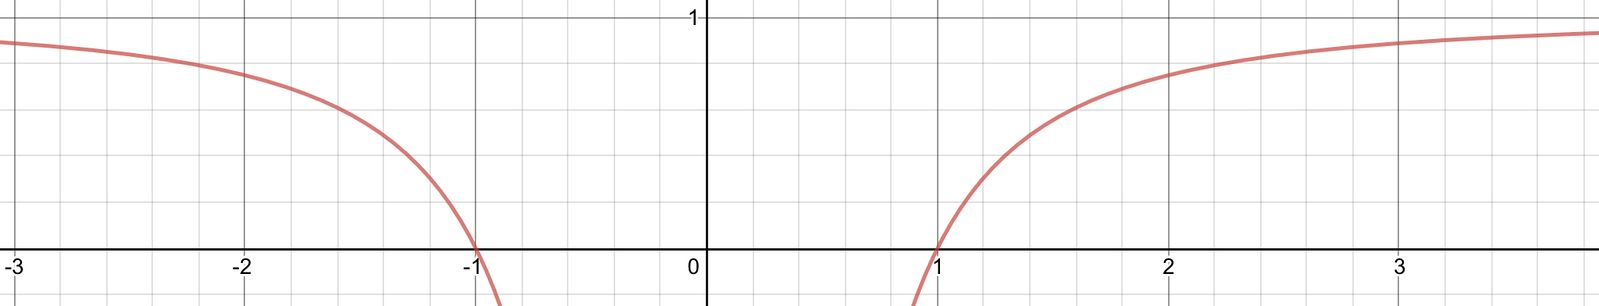
\includegraphics[width=15cm]{graph.jpeg}
\end{center}
\vspace{3mm}

\noindent \textbf{B-v)}  Since the term $\frac{2gz}{v_G^2}$ will decrease as $v_G$ increases, the radius will be less dependent on the height for high-speed tornadoes. As a result, tornadoes with relatively uniform diameter tend to have higher ground rotation speeds.
\vspace{3mm}

\noindent \textbf{C-i)} The angular velocity inside the core is constant since it behaves like a rigid body. Therefore, $v = \omega r = v_G\frac{r}{r_G}$.
\vspace{3mm}

\noindent \textbf{C-ii)}  From before, $\frac{\mathrm{d}P}{\mathrm{d}r} = \rho_{\text{air}}\frac{v^2}{r}$. Multiplying both sides by $\mathrm{d}r$ and integrating the expression from the center to a far distance away, we have: 
\[P_D - P_0 = \rho \left(\int_{0}^{r_G}\frac{v_G^2r}{r_G^2} \mathrm{d}r + \int_{r_G}^{\infty}\frac{v_G^2r}{r_G^2} \mathrm{d}r\right).\]
Evaluating and solving algebraically for $P_D$, we get $P_D = P_0 - \rho v_G^2 \approx 76.48\;\mathrm{kPa}$.
\vspace{3mm}

\noindent \textbf{C-iii)} Assuming adiabatic behavior, $P^{1 - \gamma} \propto \frac{1}{T^\gamma}$. Therefore, $$T_G = T_0\left(\frac{P_G}{P_0}\right)^{\frac{\gamma - 1}{\gamma}} \approx 4.89\;\mathrm{^{\circ} C}$$ and $$T_D= T_0\left(\frac{P_D}{P_0}\right)^{\frac{\gamma - 1}{\gamma}} \approx -6.25\;\mathrm{^{\circ} C}.$$
\vspace{3mm}

\noindent \textbf{C-iv)} The low temperature causes condensation of moisture that gets sucked into the core, which releases a lot of latent heat, a source of the tornado's energy.
\vspace{3mm}

\noindent \textbf{D-i)} We assume that the house is tightly enclosed with pressure $P_0$ inside.
By substituting $v = v_G\frac{r}{r_G}$ into $\frac{\mathrm{d}P}{\mathrm{d}r} = \rho_{\text{air}}\frac{v^2}{r}$, the following integral can be set up: 
\[\Delta P = \rho_{air}\int_{2r_G}^{\infty} \frac{v_G^2r_G^2}{r^3} \mathrm{d}r.\]
Evaluating, $\Delta P = \frac{1}{8}\rho_{air}v_G^2$. Since the lift force is $F_L = \Delta PA$, the ratio of the lift force to weight for the roof is $\frac{F_L}{F_G} = \frac{\Delta PA}{\rho_{\text{roof}}Atg} = 3.75$.
\vspace{3mm}

\noindent \textbf{D-ii)} The lift force is not much larger than the weight of the roof, most roof are mounted firmly to withstand forces many times it’s weight. Therefore, chances are the pressure difference would not cause the house to explode so soon (unless the roof is very poorly mounted). Opening windows during a tornado isn't a good idea for another reason. Flying debris is responsible for most twister-related injuries, so standing next to an opening that could potentially blast you with shards of glass and other projectiles isn’t a great idea.

\end{solution}